% Generated by ICLR_Q4.py from experiment_logs_Q4 -- Drone4D_x0set: Abstract states ($|S|$)
% Shaded band = min/max over seeds; line = median over seeds.
% Picture width is exactly \linewidth. Requires \usepackage{pgfplots}.
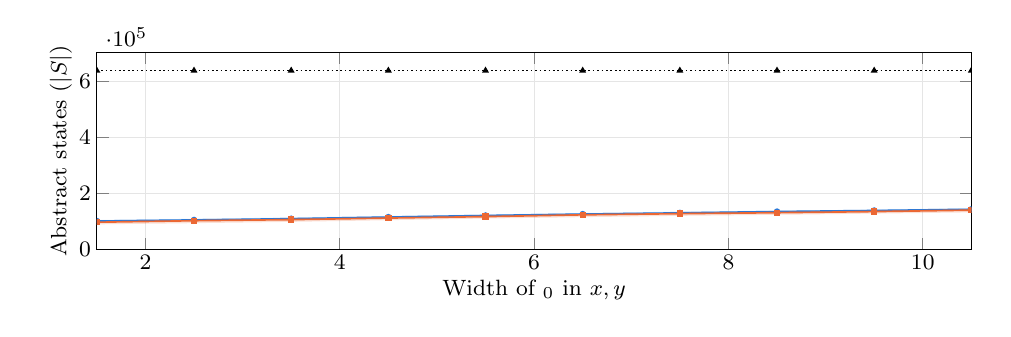
\begin{tikzpicture}[baseline=(current axis.south)]
\definecolor{q4ppo}{RGB}{42,120,214}
\definecolor{q4sac}{RGB}{235,104,52}
\definecolor{q4dense}{RGB}{0,0,0}
\begin{axis}[
    scale only axis, width=\linewidth-25pt-4pt, height=2.5cm,
    xlabel={Width of $\X_0$ in $x,y$},
    ylabel={Abstract states ($|S|$)}, ylabel style={align=center},
    xmin=1.5, xmax=10.5, xtick={2,4,6,8,10},
    ymin=0,
    grid=major, grid style={gray!20}, clip marker paths=true,
    label style={font=\footnotesize}, tick label style={font=\footnotesize, inner sep=2pt},
    xlabel shift=-2pt, ylabel shift=-3pt,  % labels close to the tick labels
]
% PPO: 5 seeds per X0 span
\addplot[draw=none, fill=q4ppo, fill opacity=0.2, forget plot] coordinates {(1.5,98744) (2.5,103375) (3.5,107424) (4.5,112760) (5.5,119166) (6.5,124791) (7.5,129688) (8.5,132625) (9.5,137618) (10.5,142700) (10.5,147256) (9.5,142704) (8.5,138887) (7.5,135526) (6.5,130372) (5.5,125180) (4.5,119773) (3.5,114423) (2.5,109788) (1.5,105379)} -- cycle;
\addplot[q4ppo, semithick, mark=*, mark size=0.85pt] coordinates {(1.5,101852) (2.5,105732) (3.5,110207) (4.5,116071) (5.5,121652) (6.5,126682) (7.5,130994) (8.5,135769) (9.5,139486) (10.5,143836)};
% SAC: 5 seeds per X0 span
\addplot[draw=none, fill=q4sac, fill opacity=0.2, forget plot] coordinates {(1.5,89969) (2.5,94202) (3.5,98888) (4.5,104859) (5.5,110774) (6.5,115750) (7.5,120421) (8.5,124158) (9.5,128485) (10.5,132828) (10.5,144613) (9.5,139754) (8.5,135710) (7.5,131505) (6.5,127182) (5.5,122306) (4.5,115567) (3.5,110532) (2.5,105015) (1.5,101244)} -- cycle;
\addplot[q4sac, semithick, mark=square*, mark size=0.85pt] coordinates {(1.5,97565) (2.5,102945) (3.5,106818) (4.5,112453) (5.5,117588) (6.5,123979) (7.5,128151) (8.5,131569) (9.5,135548) (10.5,140717)};
% Dense (single deterministic run per X0 span)
\addplot[q4dense, semithick, mark=triangle*, mark size=0.85pt, densely dotted, mark options={solid}] coordinates {(1.5,640000) (2.5,640000) (3.5,640000) (4.5,640000) (5.5,640000) (6.5,640000) (7.5,640000) (8.5,640000) (9.5,640000) (10.5,640000)};
\end{axis}
% Fix the bounding box to exactly \linewidth wide: the axis box plus the label margins
\path (current axis.south west |- current bounding box.south) ++(-25pt,0) coordinate (q4sw)
      (current axis.north east |- current bounding box.north) ++(4pt,0) coordinate (q4ne);
\pgfresetboundingbox
\useasboundingbox (q4sw) rectangle (q4ne);
\end{tikzpicture}%
